
\begin{frame}{Appendix --- The Council Race as Placebo Office}
\hypertarget{app:councilplacebo}{}
\small
The same instrument, built once from the executive design and applied to the council (vereador) race, returns a near-complete null: a large, fluid, multi-seat proportional contest absorbs the same litigation with almost no compositional trace. The asymmetry is what front-runner reinforcement predicts, since the mechanism operates on a single-winner race and has no counterpart in a multi-seat proportional one.
\smallskip
\begin{center}
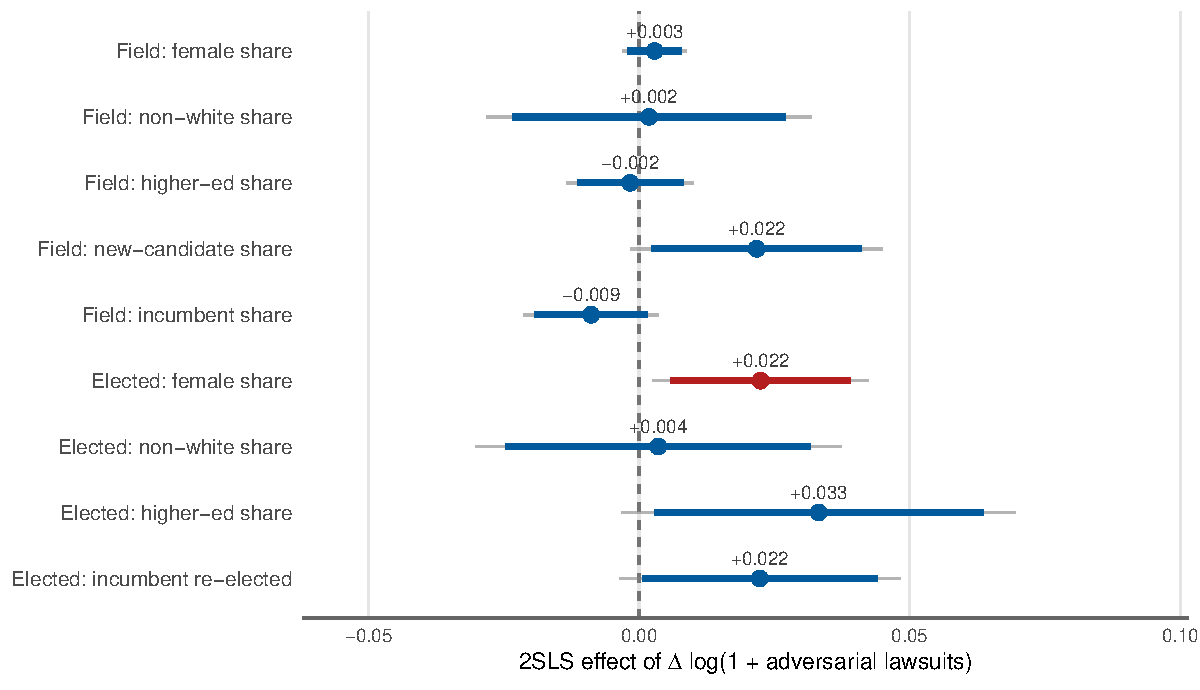
\includegraphics[width=\linewidth,height=0.42\textheight,keepaspectratio]{../figures/legislative_coefplot.pdf}
\end{center}
\smallskip
\takeaway{Of the plotted council outcomes only the elected female share clears 5\% ($\CouncilElFemaleCoef$, $p=\CouncilElFemaleP$); the elected higher-education share ($p=\CouncilElHigherEdP$) and the field's new-candidate share ($p=\CouncilNewCandP$) clear 10\%. Off the plot, the candidate pool is younger (\CouncilAgeYr~yr, $p=\CouncilAgeP$). \CouncilNSig{} of \CouncilNOutcomes{} council outcomes clear 5\%, and no multiplicity correction is computed for the council. Field size ($p=\LegCandP$) and party mix are flat.}\hfill\hyperlink{app:legislative}{\beamergotobutton{Full legislative tables}}\,\hyperlink{app:ballotcouncil}{\beamergotobutton{council ballot}}\,\hyperlink{src:voterballot}{\beamerreturnbutton{Back}}
\end{frame}
